\documentclass[11pt,letterpaper]{article}

\usepackage[margin=1in]{geometry}
\usepackage{amsmath,amssymb,amsfonts}
\usepackage{graphicx}
\usepackage{xcolor}
\usepackage{enumitem}
\usepackage{float}
\usepackage{hyperref}
\usepackage{microtype}
\usepackage{bm}

\hypersetup{
  colorlinks=true,
  linkcolor=blue!60!black,
  citecolor=blue!60!black,
  urlcolor=blue!60!black
}

\newcommand{\thet}{\bm{\theta}}
\newcommand{\R}{\mathbb{R}}
\newcommand{\E}{\mathbb{E}}
\newcommand{\Var}{\operatorname{Var}}
\newcommand{\diag}{\operatorname{diag}}
\newcommand{\tr}{\operatorname{tr}}
\newcommand{\op}{\mathrm{op}}

\title{\textbf{Optimizers, Schedulers, and Weight Decay\\
from First Principles}}
\author{}
\date{}

\begin{document}
\maketitle

\tableofcontents


%======================================================================
\newpage
\section{One Parameter in a Smooth Loss}
%======================================================================

Let $\theta\in\R$ be a scalar parameter and let $V(\theta)$ be a twice
continuously differentiable loss. At iteration $t$, denote the current
parameter by $\theta_t$, its gradient by $g_t$, the learning rate by
$\eta_t$, and the parameter displacement by $\Delta\theta_t$. Gradient
descent takes the step
\begin{equation}\label{eq:one_d_gd}
  g_t=V'(\theta_t),
  \qquad
  \Delta\theta_t=-\eta_t g_t,
  \qquad
  \theta_{t+1}=\theta_t+\Delta\theta_t.
\end{equation}
For $\eta_t>0$, the sign of $V'(\theta_t)$ gives the direction and
$\eta_t$ sets the distance.

\begin{figure}[H]
  \centering
  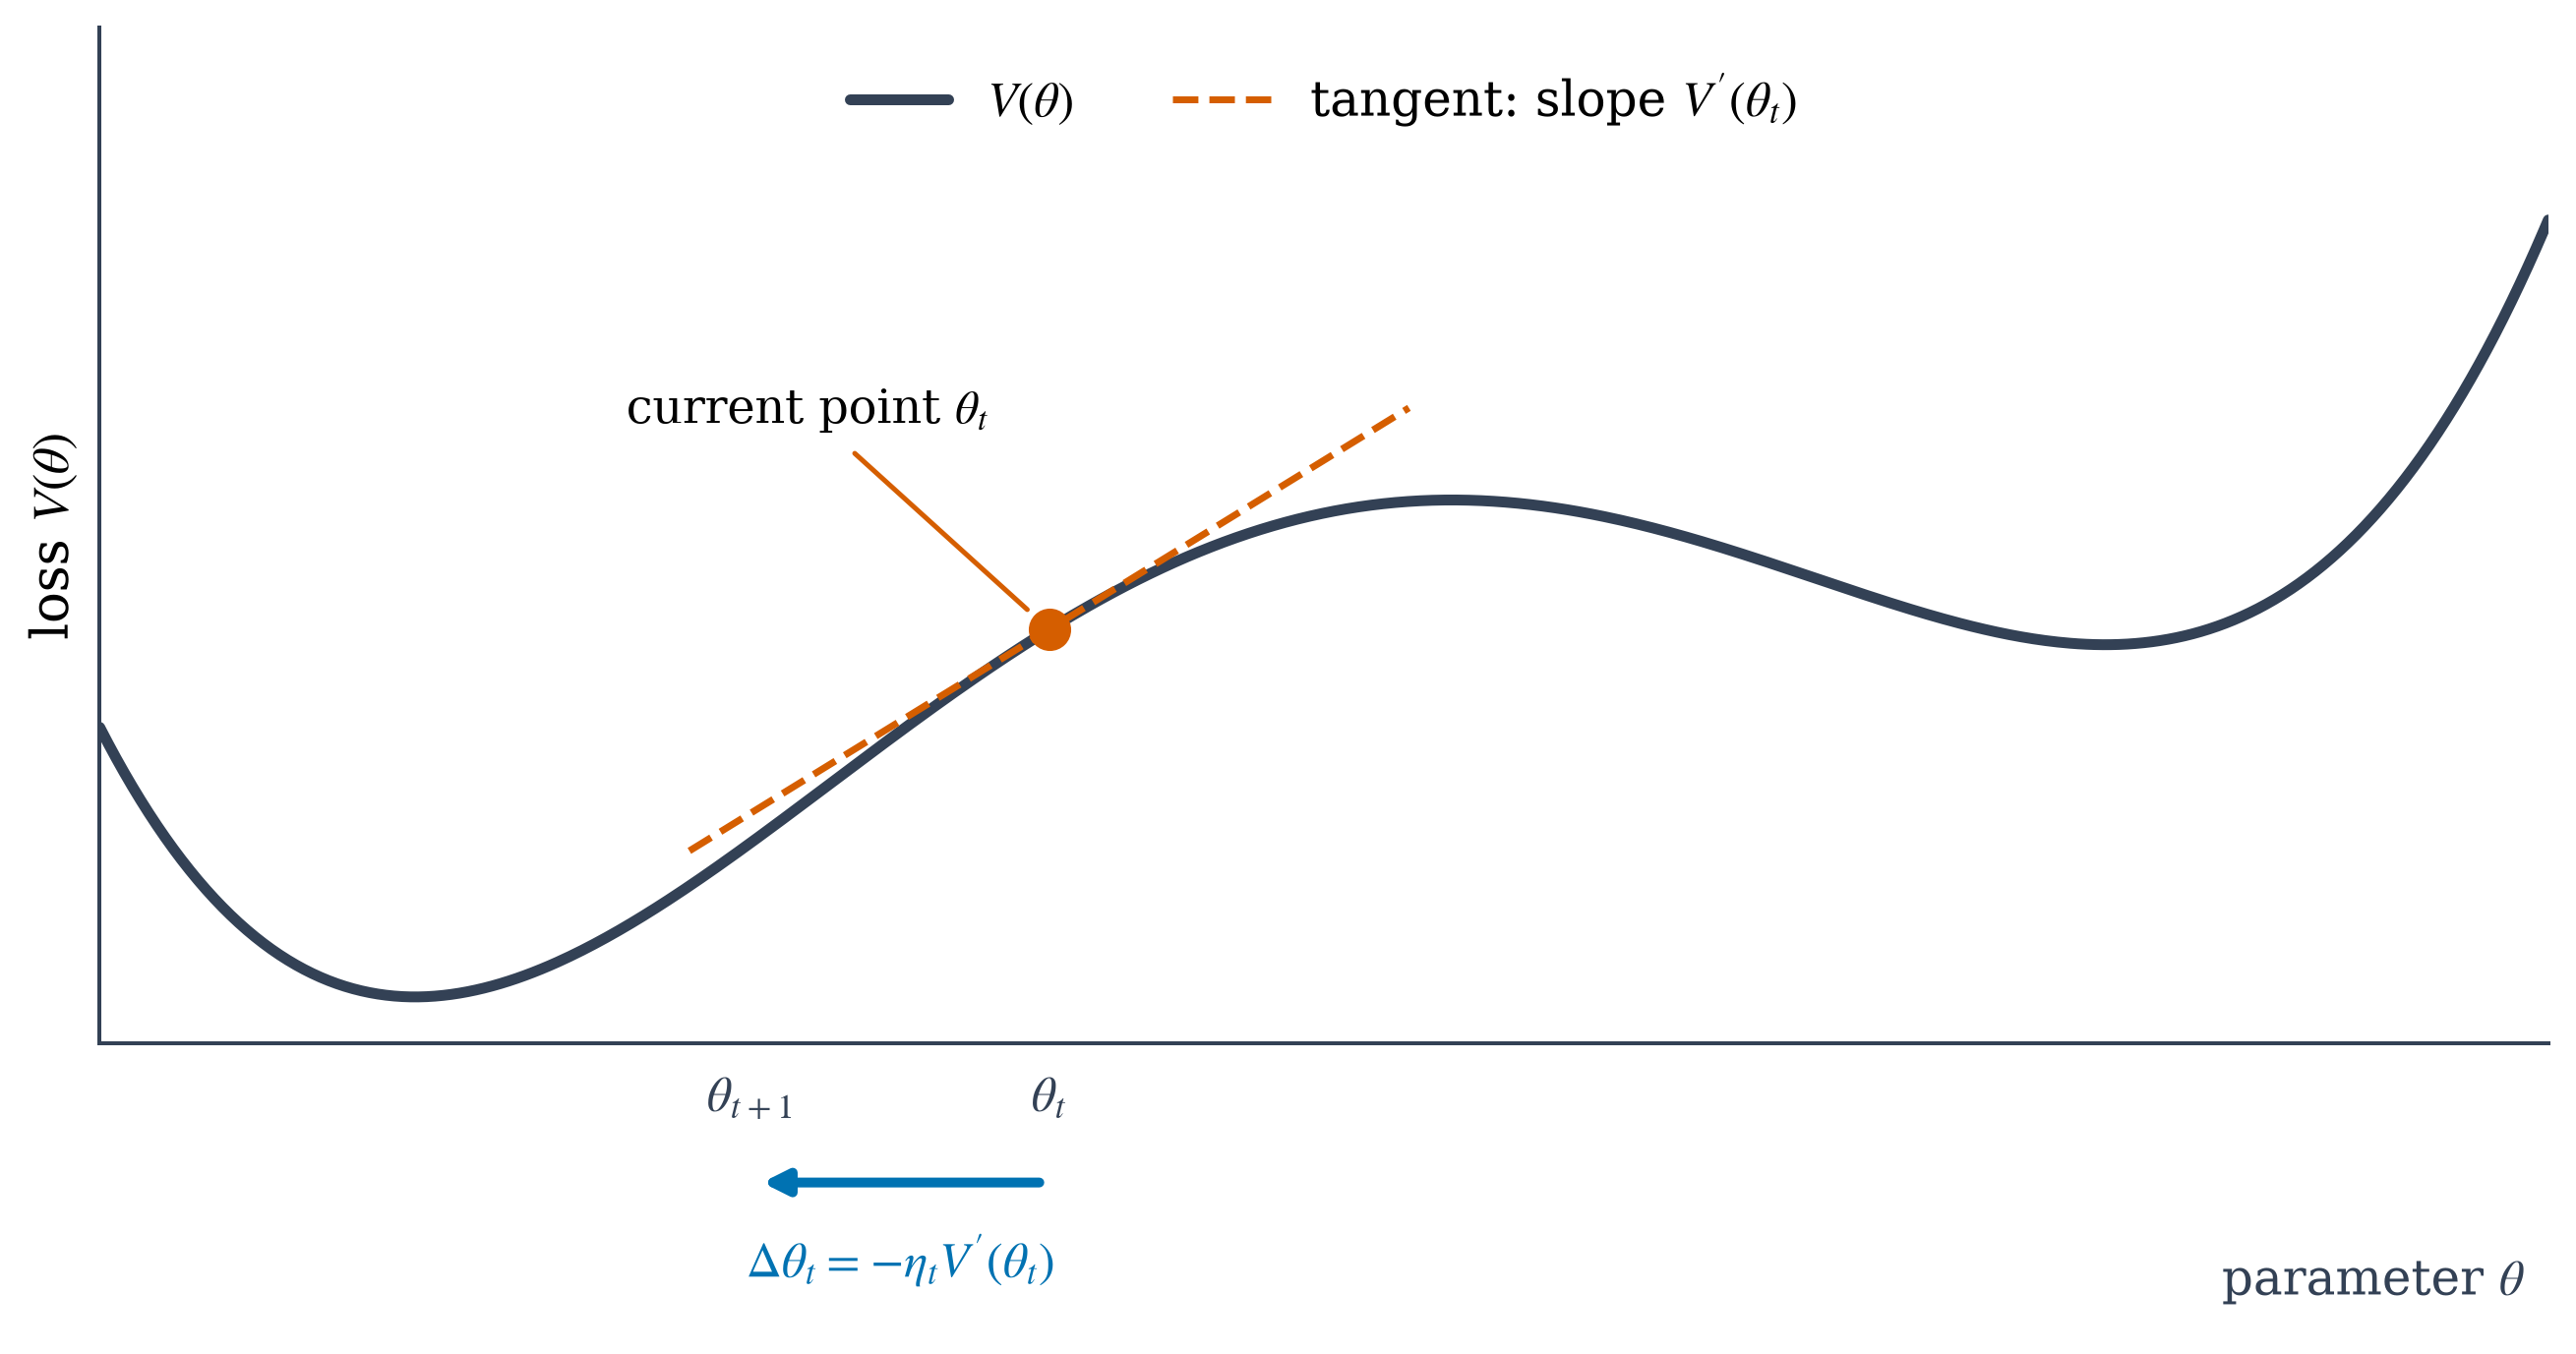
\includegraphics[width=0.78\textwidth]
    {fig_local_update.png}
  \caption{One gradient-descent step on a smooth loss. The derivative at
  $\theta_t$ is the slope of the tangent; multiplying its negative by
  $\eta_t$ gives the parameter displacement.}
  \label{fig:local_update}
\end{figure}

\paragraph{Global target and local information.}

Choose a global minimizer $\widetilde\theta$, and denote the error at iteration
$t$ by $e_t$ and the curvature at the minimizer by $\widetilde h$:
\begin{equation}
  \begin{aligned}
    \widetilde\theta&\in\arg\min_{\theta\in\R}V(\theta),
    &e_t&\equiv\theta_t-\widetilde\theta,\\
    V'(\widetilde\theta)&=0,
    &\widetilde h&\equiv V''(\widetilde\theta)\geq0.
  \end{aligned}
\end{equation}
At the position $\theta_t$ in parameter space, the current gradient $g_t$ and
local curvature $h_t$ are
\begin{equation}
  g_t=V'(\theta_t),
  \qquad
  h_t=V''(\theta_t).
\end{equation}
Both are properties of the loss surface, not choices made by the optimizer.
Substituting $\Delta\theta_t$ into \eqref{eq:one_d_gd}, the parameter update
in closed form is
\begin{equation}\label{eq:one_d_gd_closed}
  \theta_{t+1}=\theta_t-\eta_tg_t.
\end{equation}
Subtracting the fixed number $\widetilde\theta$ from both sides and using
$e_t\equiv\theta_t-\widetilde\theta$ gives the exact finite-error update
\begin{equation}\label{eq:error_update}
  e_{t+1}=e_t-\eta_tg_t.
\end{equation}
For the iteration to make progress toward the chosen minimizer, we would like
the error magnitude---the distance $|e_t|$ from $\theta_t$ to
$\widetilde\theta$---to decrease from one step to the next, so that
$|e_{t+1}|<|e_t|$. However, the algorithm cannot test this desired contraction
directly. It can evaluate $g_t$ at the current iterate, but it does not know
$e_t$, because the latter depends on the unknown minimizer $\widetilde\theta$.

The loss geometry available around the current iterate is local. In particular,
the curvature $h_t$ determines how the gradient changes, to first order, under
a small displacement $\delta\theta$:
\[
  V'(\theta_t+\delta\theta)
  =g_t+h_t\delta\theta+O(\delta\theta^2).
\]

\paragraph{Optimizer, scheduler, and weight decay.}

At iteration $t$, let $\theta_t$ be the current parameter,
$g_t=V'(\theta_t)$ the task gradient, $\mathcal O_t(g_0,\ldots,g_t)$ the
update direction produced by the optimizer, $\eta_t>0$ the learning rate
supplied by the scheduler, and $\lambda_t\geq0$ the weight-decay coefficient.
The weight-decay update is
\begin{equation}\label{eq:optimizer_scheduler_decay}
  \theta_{t+1}
  =\theta_t
   -\eta_t\mathcal O_t(g_0,\ldots,g_t)
   -\eta_t\lambda_t\theta_t.
\end{equation}
The last term, $-\eta_t\lambda_t\theta_t$, is the additional decay term. For
plain gradient descent, $\mathcal O_t(g_0,\ldots,g_t)=g_t$, so the update is
\begin{equation}\label{eq:gradient_descent_decay}
  \theta_{t+1}
  =\theta_t-\eta_tg_t-\eta_t\lambda_t\theta_t.
\end{equation}
The same term can also be generated by adding a quadratic penalty to the loss,
\begin{equation}\label{eq:regularized_potential}
  V_{\lambda_t}(\theta)
  =V(\theta)+\frac{\lambda_t}{2}\theta^2.
\end{equation}
Indeed, $V_{\lambda_t}'(\theta_t)=g_t+\lambda_t\theta_t$, and a gradient
step on $V_{\lambda_t}$ gives
\begin{align}
  \theta_{t+1}
  &=\theta_t-\eta_tV_{\lambda_t}'(\theta_t)\\
  &=\theta_t-\eta_tg_t-\eta_t\lambda_t\theta_t,
\end{align}
which is exactly Eq.~\eqref{eq:gradient_descent_decay}. Thus, for plain
gradient descent, adding the quadratic penalty to the loss and applying
weight decay directly to the parameters are algebraically equivalent.
Section~\ref{sec:weight_decay} explains when this equivalence fails and then
separates the physical effects of the two implementations.

To express the same update in terms of the optimization error, subtract
$\widetilde\theta$ from both sides:
\begin{equation}\label{eq:error_update_decay}
  \begin{aligned}
    \theta_{t+1}-\widetilde\theta
    &=\theta_t-\widetilde\theta-\eta_t(g_t+\lambda_t\theta_t),\\
    e_{t+1}
    &=e_t-\eta_tg_t-\eta_t\lambda_t(e_t+\widetilde\theta)\\
    &=(1-\eta_t\lambda_t)e_t-\eta_tg_t
      -\eta_t\lambda_t\widetilde\theta.
  \end{aligned}
\end{equation}
Equation~\eqref{eq:error_update_decay} already shows the important point:
weight decay acts on \(\theta_t=e_t+\widetilde\theta\), not on the error \(e_t\)
alone. It is centered at the parameter origin, not at the unknown minimizer,
so it cannot be interpreted as directly keeping the distance to
\(\widetilde\theta\) small. Section~\ref{sec:weight_decay} makes this distinction
explicit.

\paragraph{Local transport along the training curve.}

Let $\delta\theta_t$ denote the separation at step $t$ between two runs of
the same update rule started from nearby initial parameters. Differentiating
the gradient-descent case of \eqref{eq:optimizer_scheduler_decay} with respect
to $\theta_t$ gives its evolution to first order,
\begin{equation}\label{eq:local_tangent}
  \delta\theta_{t+1}
  =\bigl[1-\eta_t(h_t+\lambda_t)\bigr]\delta\theta_t.
\end{equation}
This equation uses only the curvature at $\theta_t$. It measures whether
neighbouring trajectories are pulled together, which is a weaker statement
than convergence of either one.

Everything so far has used a single parameter. The rest of this note needs
several, so denote the full $d$-component parameter vector by $\thet$:
\begin{equation}\label{eq:parameter_vector}
  \thet=(\theta_1,\ldots,\theta_d)\in\R^d
\end{equation}

Bold symbols denote vectors and capital letters
denote matrices, so $\nabla V(\thet)\in\R^d$ is the gradient and
$\nabla^2V(\thet)\in\R^{d\times d}$ the Hessian. Where the transport
equations below are written in index notation, Greek indices
$\mu,\nu\in\{1,\ldots,d\}$ label components, an upper index marks a vector
component and a lower index a covector component, and a repeated
upper--lower pair is summed over; $\theta^\mu$ and $\theta_\mu$ are the same
$d$ numbers written in the two positions, since the parameter space carries
the Euclidean metric.

Let $\rho^\mu(t)$ be the parameter trajectory and reserve $\lambda(t)$ for
the weight-decay coefficient.
Denote the Hessian evaluated at the current point of the trajectory by
$H^\mu{}_{\nu}(t)$:
\begin{equation}
  H^\mu{}_{\nu}(t)
  =\left.
    \frac{\partial^2 V(\thet)}
         {\partial\theta_\mu\,\partial\theta^\nu}
    \right|_{\thet=\rho(t)}.
\end{equation}
Both derivatives act on the parameter coordinates of $V$; $t$ only selects
the evaluation point $\rho(t)$.
For discrete updates, write $H_t=\nabla^2V(\thet_t)$ and let $I$ denote the
$d\times d$ identity matrix. After $N$ updates, gradient descent with
decoupled decay transports a tangent displacement according to
\begin{equation}
  \delta\thet_N
  =\bigl[I-\eta_{N-1}(H_{N-1}+\lambda_{N-1}I)\bigr]\cdots
   \bigl[I-\eta_0(H_0+\lambda_0I)\bigr]\delta\thet_0,
\end{equation}
where later steps multiply from the left. Writing this ordered product does
not establish that its norm vanishes as $N\to\infty$.

For gradient flow with learning-rate function $\eta(t)$ and decoupled-decay
coefficient $\lambda(t)$,
\begin{equation}
  \dot\rho^\mu(t)
  =-\eta(t)\left[
    \partial^\mu V\bigl(\rho(t)\bigr)
    +\lambda(t)\rho^\mu(t)
  \right].
\end{equation}
An infinitesimal displacement $\delta\theta^\mu(t)$ between nearby
trajectories obeys
\begin{equation}\label{eq:tangent_flow}
  \frac{d}{dt}\delta\theta^\mu(t)
  =-\eta(t)\left[
    H^\mu{}_{\nu}(t)+\lambda(t)\delta^\mu{}_{\nu}
  \right]\delta\theta^\nu(t),
\end{equation}
where $\delta^\mu{}_{\nu}$ is the Kronecker delta. Let $\mathcal P$ denote
time ordering, with later times multiplying from the left, and let
$U_\rho(t,0)$ denote the resulting transport operator. The solution is
\begin{equation}\label{eq:path_ordered_transport}
  \begin{aligned}
    \delta\thet(t)&=U_\rho(t,0)\delta\thet(0),\\
    U_\rho(t,0)
      &=\mathcal P\exp\!\left[
        -\int_0^t\eta(s)\bigl(H(s)+\lambda(s)I\bigr)\,ds
      \right].
  \end{aligned}
\end{equation}
This ordering is required because
$H(t_1)$ and $H(t_2)$ need not commute.
Since $\lambda(t)I$ commutes with every Hessian, the propagator factors as
\begin{equation}
  U_\rho(t,0)
  =\exp\!\left[-\int_0^t\eta(s)\lambda(s)\,ds\right]
  \mathcal P\exp\!\left[-\int_0^t\eta(s)H(s)\,ds\right].
\end{equation}
The first factor is weight-decay damping. The ordered factor records how a
local perturbation changes along the chosen trajectory. Neither factor proves
that the trajectory approaches the global minimizer.

Figure~\ref{fig:transport} shows both objects on a surface with genuinely
varying curvature. The valley floor is a parabola, so the Hessian
eigenvectors rotate as the curve advances and $H(t_1)$ and $H(t_2)$ do not
commute; path ordering in \eqref{eq:path_ordered_transport} is therefore not
a formality. The displacement is compressed quickly in the stiff direction
transverse to the valley and then slowly along the valley floor, so the
transported norm falls faster than the weight-decay factor alone. The gap
between the two curves in panel~(c) is the contribution of the ordered
factor.

\begin{figure}[H]
  \centering
  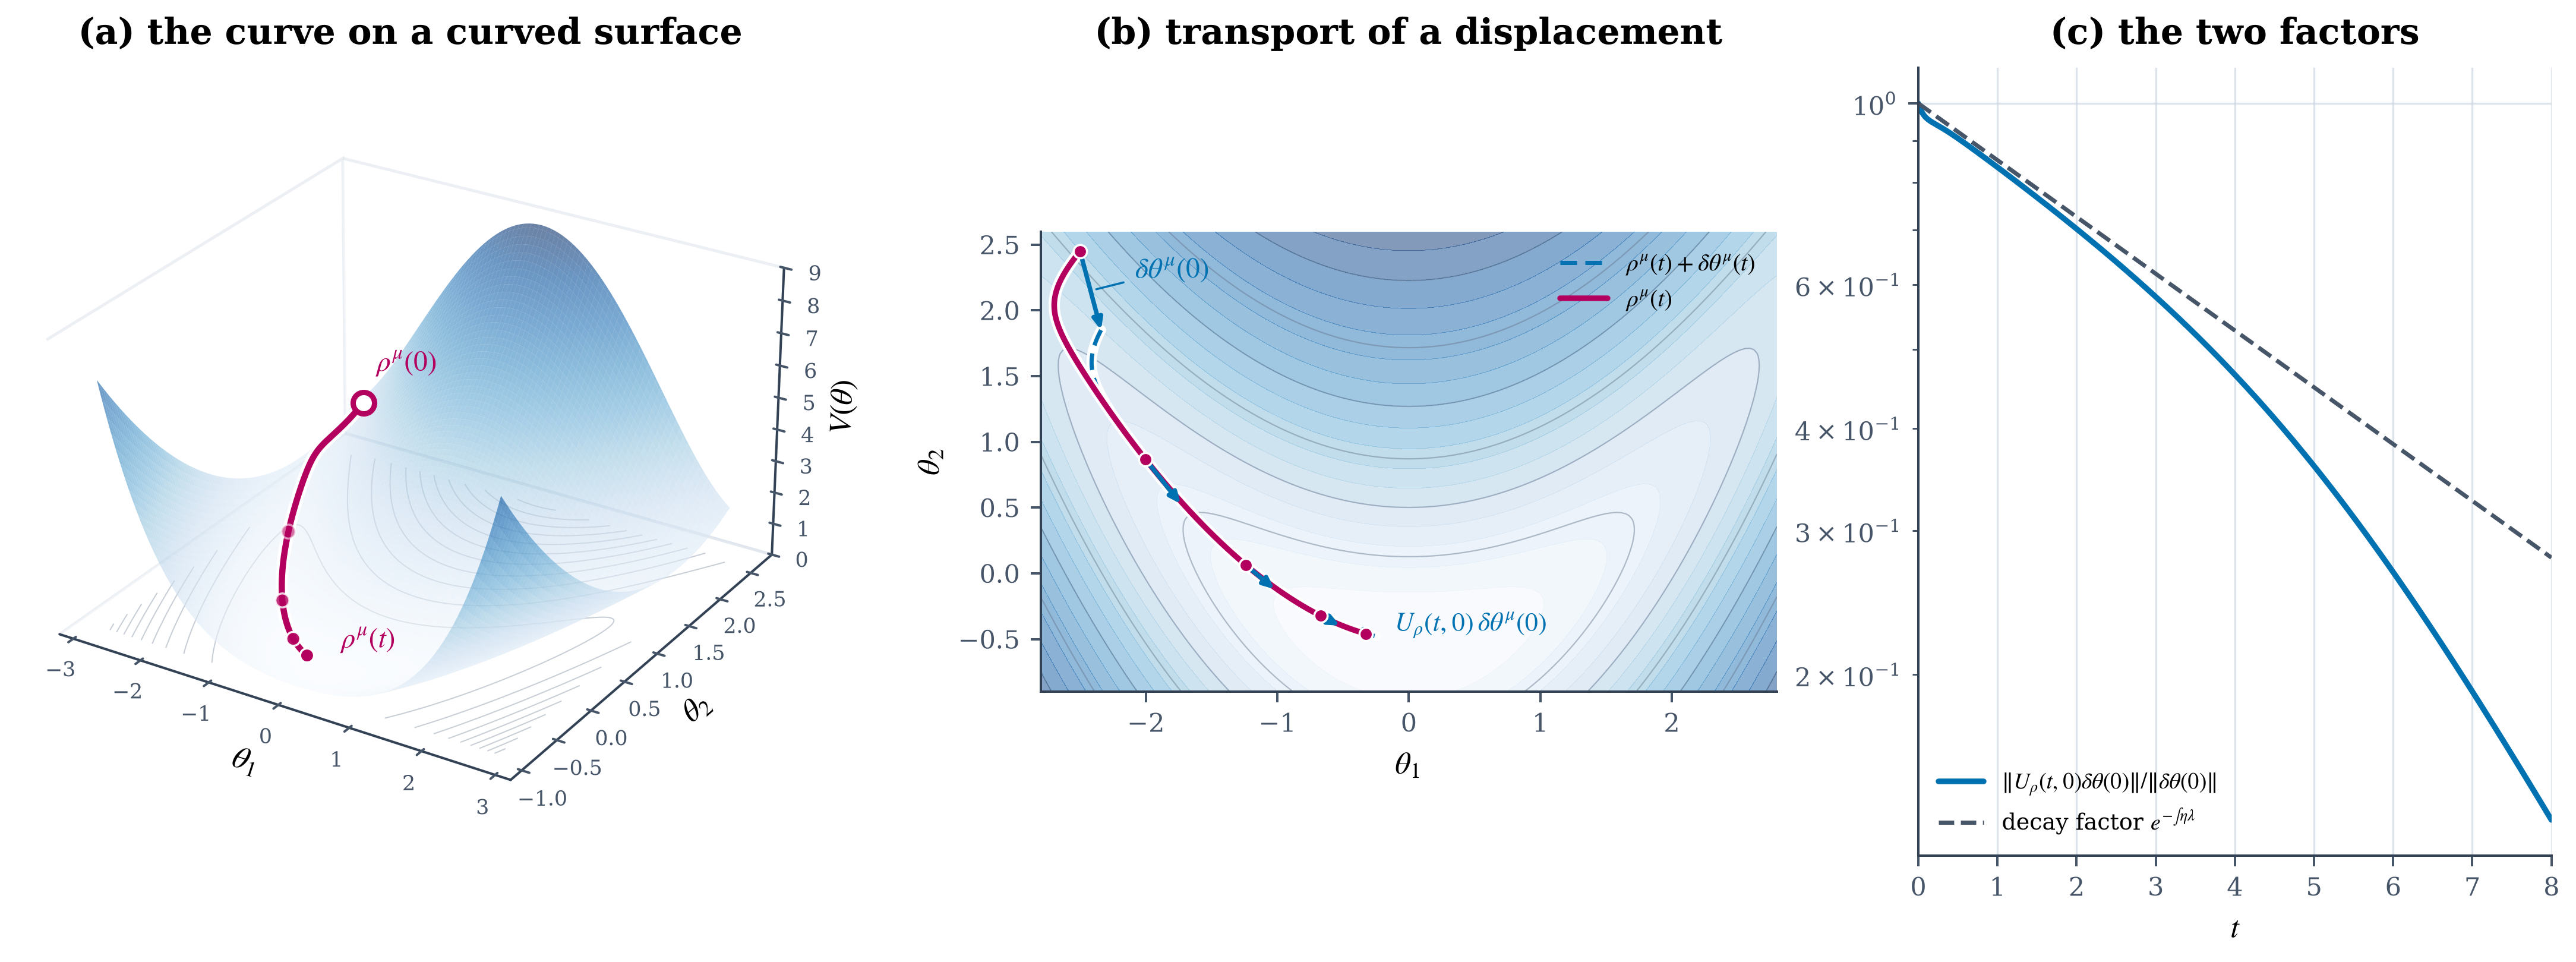
\includegraphics[width=\textwidth]
    {fig_transport.png}
  \caption{Local transport along the training curve. (a) The curve
  $\rho^\mu(t)$ of gradient flow with decay, drawn on a bent valley whose
  curvature varies from point to point. (b) The same curve seen from above,
  with the displacement $\delta\theta^\mu(t)=U_\rho(t,0)\delta\theta^\mu(0)$
  at five times, and a neighbouring trajectory started at
  $\rho^\mu(0)+\delta\theta^\mu(0)$. (c) The transported norm against the
  weight-decay factor $\exp[-\int_0^t\eta\lambda\,ds]$ of the factorization
  above; their ratio is the ordered Hessian factor. Here $\eta=1$ and
  $\lambda=0.16$ are held constant so that only the geometry varies.}
  \label{fig:transport}
\end{figure}


\newpage
\section{Three Failure Modes, Three Optimizers}
%======================================================================

To isolate the optimizer, hold the learning rate fixed at \(\eta>0\) and set
weight decay to zero. The baseline is gradient descent:
\begin{equation}\label{eq:gradient_descent_baseline}
  g_t=V'(\theta_t),
  \qquad
  u_t=g_t,
  \qquad
  \theta_{t+1}=\theta_t-\eta u_t
  =\theta_t-\eta V'(\theta_t).
\end{equation}
The three optimizers below are not three generic upgrades to this rule. Each
targets a different mismatch: momentum acts on patterns across \emph{time},
Adam acts on scales across parameter \emph{coordinates}, and Muon acts on the
singular modes of a parameter \emph{matrix}. The examples make those
distinctions exact.

\subsection{Stiff versus soft curvature: momentum}

\paragraph{Failure.}
A single learning rate must be small enough for the sharpest direction of the
loss, even when that makes progress along flatter directions painfully slow.
Let $x$ be the stiff coordinate with curvature $h_{\rm stiff}$ and let $y$
be the soft coordinate with curvature $h_{\rm soft}$. The simplest example
is the anisotropic quadratic
\begin{equation}\label{eq:momentum_anisotropic}
  V(x,y)=\frac12\left(h_{\rm stiff}x^2+h_{\rm soft}y^2\right),
  \qquad h_{\rm stiff}\gg h_{\rm soft}>0.
\end{equation}
Gradient descent gives two independent updates,
\begin{equation}\label{eq:anisotropic_gd_modes}
  x_{t+1}=(1-\eta h_{\rm stiff})x_t,
  \qquad
  y_{t+1}=(1-\eta h_{\rm soft})y_t.
\end{equation}
The stiff coordinate changes by the fraction \(\eta h_{\rm stiff}\) on each
step; the soft coordinate changes only by \(\eta h_{\rm soft}\). Increasing
\(\eta\) enough to move quickly along \(y\) makes \(x\) overshoot or diverge.
Decreasing it to control \(x\) leaves \(y\) crawling. A scheduler cannot
remove this simultaneous conflict: at any one step it still multiplies both
directions by the same scalar.

\paragraph{Fix: reinforce persistence, cancel oscillation.}
Momentum does one simple thing: gradients with the same sign add, while
gradients with alternating signs cancel. Let
\(\bm g_t\equiv\nabla V(\thet_t)\) be the gradient, let \(\bm v_{t+1}\) be
the parameter displacement at step \(t\), and let \(\beta\) be the momentum
coefficient. The update is
\begin{equation}\label{eq:momentum_velocity}
  \bm v_{t+1}=\beta\bm v_t-\eta\bm g_t,
  \qquad
  \thet_{t+1}=\thet_t+\bm v_{t+1},
  \qquad 0\leq\beta<1.
\end{equation}

\paragraph{Why the buffer has the form ``\(\beta\) old
\(+\,(1-\beta)\) new.''}
The velocity convention above hides a simple moving average. Define the
normalized momentum buffer \(\bm m_t\) by rescaling the displacement:
\begin{equation}
  \bm m_t\equiv-\frac{1-\beta}{\eta}\bm v_{t+1}.
\end{equation}
Then the first equation in \eqref{eq:momentum_velocity} becomes
\begin{equation}\label{eq:momentum_ema}
  \bm m_t
  =\beta\bm m_{t-1}+(1-\beta)\bm g_t.
\end{equation}
The coefficients add to one, so this is an average rather than a growing
total. An even clearer rearrangement is
\begin{equation}
  \bm m_t-\bm m_{t-1}
  =(1-\beta)(\bm g_t-\bm m_{t-1}).
\end{equation}
At every step, the buffer moves a fraction \(1-\beta\) from its old value
toward the new gradient. A direct sum \(\bm m_t=\bm m_{t-1}+\bm g_t\) would
grow without bound for a constant gradient and would never forget stale
directions. The weighted average stays on the gradient's scale, forgets an
observation by a factor \(\beta\) per step, and has an effective memory of
roughly \(1/(1-\beta)\) steps. The normalized buffer \(\bm m_t\) and the
stored displacement \(\bm v_{t+1}\) contain exactly the same history; they
differ only by the fixed scale \(-\eta/(1-\beta)\).

If \(\bm v_0=0\), unrolling the first equation gives
\begin{equation}
  \bm v_{t+1}
  =-\eta\sum_{k=0}^{t}\beta^k\bm g_{t-k}.
\end{equation}
For equally sized recent gradients, the two limiting cases are
\begin{equation}
  \begin{aligned}
    \bm g_{t-k}=\bm g_t
    &\quad\Longrightarrow\quad
    \bm v_{t+1}\longrightarrow
      -\frac{\eta}{1-\beta}\bm g_t,
    &&\text{same sign: accelerate},\\
    \bm g_{t-k}=(-1)^k\bm g_t
    &\quad\Longrightarrow\quad
    \bm v_{t+1}\longrightarrow
      -\frac{\eta}{1+\beta}\bm g_t,
    &&\text{alternating sign: suppress}.
  \end{aligned}
\end{equation}
Compared with the gradient-descent step \(-\eta\bm g_t\), the first step is
larger because \(1/(1-\beta)>1\), while the second is smaller because
\(1/(1+\beta)<1\). This is the entire mechanism. The stored displacement is a
discrete velocity that persists from one step to the next, hence the name
\emph{momentum}.

Since \(\bm v_t=\thet_t-\thet_{t-1}\), direct substitution gives the same rule
using parameters only:
\begin{equation}\label{eq:momentum_update}
  \begin{aligned}
    \thet_{t+1}
      &=\thet_t+\bm v_{t+1}\\
      &=\thet_t+\beta\bm v_t-\eta\bm g_t\\
      &=\thet_t-\eta\nabla V(\thet_t)
        +\beta(\thet_t-\thet_{t-1}).
  \end{aligned}
\end{equation}

\paragraph{From the last term to a decay factor.}
In a quadratic direction with curvature \(h\), the coefficients are constant
and the error obeys
\begin{equation}\label{eq:momentum_error}
  e_{t+1}=(1+\beta-\eta h)e_t-\beta e_{t-1}.
\end{equation}
To find how much the error is multiplied from one step to the next, try
\(e_t=r^t\). Plugging this form into the recurrence gives
\begin{equation}
  r^{t+1}
  =(1+\beta-\eta h)r^t-\beta r^{t-1}.
\end{equation}
Dividing by \(r^{t-1}\) and moving everything to the left gives
\begin{equation}\label{eq:momentum_characteristic}
  r^2-(1+\beta-\eta h)r+\beta=0.
\end{equation}
Each root \(r\) is a possible per-step error multiplier. Its magnitude tells
how fast that mode shrinks: smaller \(\lvert r\rvert\) means faster decay. Its
sign tells whether the error stays on the same side of the minimum
\((r>0)\) or alternates sides \((r<0)\).

Without momentum, \(\beta=0\), so the equation factors as
\begin{equation}
  r\bigl[r-(1-\eta h)\bigr]=0.
\end{equation}
The lasting root is exactly the gradient-descent multiplier
\(r=1-\eta h\). With momentum, \(\beta>0\), the last term changes this linear
condition into a quadratic one. The two roots of that quadratic now determine
the decay.

\paragraph{Exact \(2/3\) example.}
Take \(h_{\rm stiff}=25\) and \(h_{\rm soft}=1\). Denote the gradient-descent
multipliers in the two directions by \(r_{\rm stiff}\) and
\(r_{\rm soft}\):
\begin{equation}
  r_{\rm stiff}=1-25\eta,
  \qquad
  r_{\rm soft}=1-\eta.
\end{equation}
The best single \(\eta\) makes their magnitudes equal, with the stiff
multiplier negative and the soft multiplier positive, because reducing one
farther would enlarge the other:
\begin{equation}
  25\eta-1=1-\eta
  \quad\Longrightarrow\quad
  \eta=\frac1{13}.
\end{equation}
At this value,
\begin{equation}
  r_{\rm stiff}=-\frac{12}{13},
  \qquad
  r_{\rm soft}=\frac{12}{13}.
\end{equation}
Thus the stiff error alternates sides and the soft error does not, but both
shrink with the slow magnitude \(12/13\simeq0.923\). No other constant scalar
\(\eta\) gives a smaller worst-case magnitude.

For momentum, choose \(\eta=1/9\) and \(\beta=4/9\).
For the stiff direction,
\begin{equation}
  1+\beta-\eta h
  =1+\frac49-\frac{25}{9}
  =-\frac43,
\end{equation}
so Equation~\eqref{eq:momentum_characteristic} becomes
\begin{equation}
  r^2+\frac43r+\frac49
  =\left(r+\frac23\right)^2=0.
\end{equation}
The stiff root is \(r=-2/3\): the error still alternates sides, but its
exponential magnitude is now \(2/3\) instead of \(12/13\).

For the soft direction,
\begin{equation}
  1+\beta-\eta h
  =1+\frac49-\frac19
  =\frac43,
\end{equation}
and the characteristic equation becomes
\begin{equation}
  r^2-\frac43r+\frac49
  =\left(r-\frac23\right)^2=0.
\end{equation}
The soft root is \(r=+2/3\): the error stays on the same side and has the same
exponential magnitude \(2/3\). The roots are repeated, so the exact solutions
may also contain a prefactor linear in \(t\), but their exponential base is
still \(2/3\). Momentum has therefore reduced the common exponential factor
from \(12/13\) to \(2/3\).

Momentum is not a curvature inverse. Its benefit depends on gradients having
useful temporal correlation; stale history can hurt when the descent direction
changes abruptly.

\subsection{Persistent coordinate-scale imbalance: Adam}

\paragraph{Failure.}
A large gradient component does not always mean that its parameter should move
farther. It may simply reflect the units or parameterization of that
coordinate. If the imbalance persists, a single learning rate gives the large
component most of every step.

Assume two coordinates require comparable progress, but their gradients have
the same \(100{:}1\) scale difference over a horizon of \(T\) successive
steps:
\begin{equation}\label{eq:adam_scale_example}
  \bm g_1=\bm g_2=\cdots=\bm g_T
  =\begin{pmatrix}100\\1\end{pmatrix}.
\end{equation}
Gradient descent moves the first coordinate one hundred times farther. A
scheduler changes only the common multiplier. Momentum sums proportional
vectors and therefore preserves the same ratio.

\paragraph{Fix: keep momentum, then normalize each coordinate.}
Adam stands for \emph{Adaptive Moment Estimation}. It builds directly on
momentum rather than replacing it. Its first buffer is exactly the momentum
average \eqref{eq:momentum_ema}, with \(\beta\) renamed \(\beta_1\):
\begin{equation}
  \bm m_t
  =\beta_1\bm m_{t-1}+(1-\beta_1)\bm g_t,
  \qquad \bm m_0=0.
\end{equation}
Thus Adam inherits momentum's temporal filtering: same-sign gradients
reinforce one another and alternating-sign gradients cancel.

Adam then adds the second-moment buffer \(\bm s_t\): a separate running
scale for every coordinate, with decay coefficient \(\beta_2\):
\begin{equation}
  \bm s_t
  =\beta_2\bm s_{t-1}
   +(1-\beta_2)(\bm g_t\odot\bm g_t),
  \qquad \bm s_0=0.
\end{equation}
Here \(\odot\) means elementwise multiplication. The first buffer
\(\bm m_t\) remembers the signed direction, exactly as momentum does; the
second buffer \(\bm s_t\) remembers the squared size of each coordinate.
Thus \(\beta_1\) controls direction memory and \(\beta_2\) controls scale
memory, with \(0\leq\beta_1,\beta_2<1\).
Because both buffers start at zero, their weights do not yet sum to one. For a
constant gradient \(\bm g\), for example,
\begin{equation}
  \bm m_t
  =(1-\beta_1)\sum_{k=0}^{t-1}\beta_1^k\bm g
  =(1-\beta_1^t)\bm g.
\end{equation}
The symbol \(\beta_1^t\) is simply \(\beta_1\) raised to the \(t\)-th power;
the same calculation gives \(1-\beta_2^t\) for the squared-gradient buffer.
Dividing out these missing factors gives the bias-corrected first moment
\(\widehat{\bm m}_t\) and second moment \(\widehat{\bm s}_t\):
\begin{equation}\label{eq:bias_correction}
  \widehat{\bm m}_t=\frac{\bm m_t}{1-\beta_1^{\,t}},
  \qquad
  \widehat{\bm s}_t=\frac{\bm s_t}{1-\beta_2^{\,t}}.
\end{equation}
With numerical stabilizer \(\epsilon>0\), Adam uses the full update
\begin{equation}\label{eq:adam_step}
  \thet_{t+1}
  =\thet_t-\eta\frac{\widehat{\bm m}_t}
    {\sqrt{\widehat{\bm s}_t}+\epsilon},
\end{equation}
where division and square root act coordinate by coordinate; the stabilizer
prevents division by zero.

The construction is now explicit: the numerator is momentum's smoothed,
signed direction, and the denominator is Adam's new coordinate-wise
root-mean-square scale. Adam keeps the acceleration/cancellation mechanism of
momentum, then prevents a persistently large coordinate from dominating merely
because its gradients are measured on a larger scale.

\paragraph{Exact example.}
For the repeated gradient \eqref{eq:adam_scale_example}, bias correction gives
\(\widehat{\bm m}_t=\bm g_t\) and
\(\widehat{\bm s}_t=\bm g_t\odot\bm g_t\). Neglecting \(\epsilon\),
\begin{equation}
  \frac{\widehat{\bm m}_t}{\sqrt{\widehat{\bm s}_t}}
  =\begin{pmatrix}1\\1\end{pmatrix},
  \qquad
  \Delta\thet_t=-\eta\begin{pmatrix}1\\1\end{pmatrix}.
\end{equation}
Adam removes the \(100{:}1\) scale imbalance exactly in this example.

Adam's coordinate-wise rescaling can be written as the diagonal
preconditioner \(P_t\):
\begin{equation}\label{eq:adam_preconditioner}
  P_t=\diag\!\left(
    \frac{1}{\sqrt{\widehat s_{t,i}}+\epsilon}
  \right)_{i=1}^{d}.
\end{equation}
Here \(\widehat s_{t,i}\) is coordinate \(i\) of
\(\widehat{\bm s}_t\). The matrix is built from gradient history, not from
the Hessian. Adam sees
the chosen coordinate axes but not correlations between coordinates, so it is
not a general cure for curvature anisotropy. A one-off spike also provides
weak evidence for rescaling; the case for Adam is a persistent, interpretable
scale mismatch.

AdamW means Adam with \emph{decoupled weight decay}. It uses the same adaptive
moments and the same coordinate-wise step as Adam. The only difference is
where shrinkage is applied: an \(L_2\) penalty enters the gradient and hence
the two moment buffers, whereas AdamW applies weight decay directly to the
parameters, outside those buffers. Section~\ref{sec:weight_decay} derives the
difference.


\subsection{Spectral imbalance in a matrix update: Muon}

\paragraph{Failure.}
A matrix has meaningful directions that are combinations of its entries.
Adam normalizes individual entries; it does not directly normalize those
matrix directions. The distinction is explicit for the matrix gradient \(G\):

\begin{equation}\label{eq:muon_matrix_example}
  G=\frac12\begin{pmatrix}101&99\\99&101\end{pmatrix}.
\end{equation}
Instead of inspecting its four entries, apply \(G\) to the two orthogonal
directions \(\bm q_+\) and \(\bm q_-\):
\begin{equation}
  \bm q_+=\frac1{\sqrt2}\begin{pmatrix}1\\1\end{pmatrix},
  \qquad
  \bm q_-=\frac1{\sqrt2}\begin{pmatrix}1\\-1\end{pmatrix}.
\end{equation}
Direct multiplication gives
\begin{equation}
  G\bm q_+=100\bm q_+,
  \qquad
  G\bm q_-=\bm q_-.
\end{equation}
Thus \(G\) is one hundred times stronger along the common direction
\(\bm q_+\) than along the difference direction \(\bm q_-\). These are its
two singular modes, with singular values \(100\) and \(1\). For parameter
matrix \(W\), SGD uses the update \(\Delta W=-\eta G\), so it preserves that
\(100{:}1\) imbalance.

For a constant \(G\) and negligible \(\epsilon\), Adam normalizes all four
positive entries separately. Denote its matrix response by \(A\):
\begin{equation}
  A=\begin{pmatrix}1&1\\1&1\end{pmatrix}.
\end{equation}
Apply this response to the same two directions:
\begin{equation}
  A\bm q_+=2\bm q_+,
  \qquad
  A\bm q_-=0.
\end{equation}
Adam has not merely reduced the \(100{:}1\) imbalance. In this example, its
entrywise normalization has deleted the difference mode completely. The
reason is simple: Adam normalized in the entry basis, while the meaningful
directions are \(\bm q_+\) and \(\bm q_-\).

\paragraph{Fix: normalize matrix modes instead of entries.}
Muon first forms a momentum matrix \(M_t\), so it retains the same temporal
filtering as momentum and Adam. It then uses a singular-value decomposition
with left singular-vector matrix \(U\), diagonal singular-value matrix
\(\Sigma\), and right singular-vector matrix \(Z\):
\begin{equation}\label{eq:svd}
  M_t=U\Sigma Z^T,
  \qquad
  \Sigma=\diag(\sigma_1,\ldots,\sigma_r),
  \qquad
  \sigma_i>0.
\end{equation}
Here \(r\) is the rank of \(M_t\). For singular mode \(i\), the input
direction \(\bm z_i\) is sent to the output direction \(\bm u_i\) with
strength \(\sigma_i\):
\begin{equation}
  M_t\bm z_i=\sigma_i\bm u_i.
\end{equation}
Idealized Muon keeps the directions but replaces every nonzero strength by
one, giving the polar factor \(UZ^T\) and matrix update \(\Delta W_t\):
\begin{equation}\label{eq:muon_polar}
  M_t\longmapsto UZ^T,
  \qquad
  (UZ^T)\bm z_i=\bm u_i,
  \qquad
  \Delta W_t=-\eta UZ^T.
\end{equation}
The essential contrast is
now precise: Adam normalizes entries, whereas Muon normalizes singular modes.

\paragraph{Exact example.}
For \eqref{eq:muon_matrix_example}, the input and output directions are both
\(\bm q_+\) and \(\bm q_-\), and the singular values are \(100\) and \(1\).
Muon replaces those two values by \(1\) and \(1\), so its response is
\begin{equation}
  UZ^T=I,
  \qquad
  I\bm q_+=\bm q_+,
  \qquad
  I\bm q_-=\bm q_-.
\end{equation}
The three optimizers therefore produce mode strengths
\begin{equation}
  \begin{array}{c|cc}
    &\bm q_+&\bm q_-\\ \hline
    \text{SGD}&100&1\\
    \text{Adam, entrywise}&2&0\\
    \text{Muon}&1&1
  \end{array}
\end{equation}
Muon removes the \(100{:}1\) imbalance without discarding either direction.

Muon is not a Hessian inverse, and it does not make the parameter matrix
\(W\) orthogonal; it changes only the update. For a vector there is only one
singular mode, so the operation reduces to ordinary vector normalization. The
polar factor can be approximated with a Newton--Schulz polynomial instead of
computing \eqref{eq:svd} explicitly.

%======================================================================
\newpage
\section{Learning-Rate Schedules: Why Warm-Up and Warm-Down}
%======================================================================

A learning-rate scheduler cannot correct an update direction; it only changes
the distance traveled in that direction. At iteration \(t\), let \(\eta_t\)
denote the learning rate and let \(\eta_{\max}\) denote its peak value. A
constant-rate run keeps \(\eta_t=\eta_{\max}\) throughout training. Warm-up
starts below the peak and raises the rate during the first part of training,
whereas warm-down lowers the rate during the final part.
Figure~\ref{fig:learning_rate_schedule} compares the three policies before
the warm-up and warm-down mechanisms are examined separately.

\begin{figure}[H]
  \centering
  \includegraphics[width=0.72\textwidth]{%
    fig_learning_rate_schedule.png}
  \caption{(a) Learning-rate histories. A constant rate makes no
  stage-dependent adjustment; warm-up limits early steps, whereas warm-down
  reduces late motion.}
  \label{fig:learning_rate_schedule}
\end{figure}
For the late-training noise mechanism, consider one noisy quadratic mode. Let
\(\widehat g_t\) be its minibatch gradient, \(e_t\) its error, \(h_t\) its
positive curvature, \(\xi_t\) the minibatch noise, \(B\) the batch size, and
\(\sigma_t^2\) the noise scale. First separate signal from noise:
\begin{equation}\label{eq:scheduler_gradient}
  \widehat g_t=h_t e_t+\xi_t.
\end{equation}
Here \(h_t e_t\) is the local deterministic gradient and \(\xi_t\) is the
minibatch fluctuation.

Assume that this fluctuation is conditionally unbiased and has conditional
variance \(\sigma_t^2/B\):
\begin{equation}\label{eq:scheduler_noise}
  \E[\xi_t\mid e_t]=0,
  \qquad
  \E[\xi_t^2\mid e_t]=\frac{\sigma_t^2}{B}.
\end{equation}
The first relation removes noise-induced drift; the second sets the kick size
and its batch-size dependence.

Substitution into one gradient-descent step gives
\begin{equation}\label{eq:scheduler_error_update}
  e_{t+1}=(1-\eta_t h_t)e_t-\eta_t\xi_t.
\end{equation}
The first term is the local response; the second is the current stochastic
kick.

Squaring and conditioning on the current error removes the cross term by
conditional unbiasedness:
\begin{equation}\label{eq:scheduler_suppression}
  \E[e_{t+1}^2\mid e_t]
  =(1-\eta_t h_t)^2e_t^2
  +\eta_t^2\frac{\sigma_t^2}{B}.
\end{equation}
The two terms measure deterministic transport and injected mean-square noise.
A schedule scales both but does not improve the gradient itself; this remains
a local diagnostic model.

\subsection{Beginning of training: keep the first updates local}

At initialization, the gradient describes only the immediate neighborhood of
the initial parameters. The peak rate can jump into a region with different
activations, curvature, and gradient scale, effectively extrapolating local
information into a new initialization. Figure~\ref{fig:learning_rate_warmup}
contrasts this nonlocal jump with the short warm-up update inside the dashed
neighborhood. Warm-up therefore acts as a temporary trust-region mechanism
while network scales and optimizer state become calibrated; it does not
guarantee that training remains in one basin.

\begin{figure}[H]
  \centering
  \includegraphics[width=0.72\textwidth]{%
    fig_learning_rate_warmup.png}
  \caption{(b) The initial gradient describes a local loss profile. From the
  same starting point and descent direction, the warm-up step remains inside
  the indicated neighborhood, whereas the constant peak rate extrapolates the
  local direction into a region with a different loss profile.}
  \label{fig:learning_rate_warmup}
\end{figure}

Once a local curvature mode is meaningful, the quadratic model gives a more
specific stability test. Ignoring noise, its error is multiplied by
\(1-\eta_t h_t\) and contracts only when
\begin{equation}\label{eq:warmup_stability}
  |1-\eta_t h_t|<1
  \qquad\Longleftrightarrow\qquad
  0<\eta_t h_t<2.
\end{equation}
If the peak rate violates this bound for an early sharp mode, warm-up also
prevents local amplification. It suppresses the stochastic-kick variance
\(\eta_t^2\sigma_t^2/B\) at the same time. If the full-rate update is already
both local and stable from the first step, these arguments alone do not
require warm-up.

\subsection{End of training: small deterministic signal and persistent noise}

Near a basin, the loss landscape need not become flat. Instead, the error
\(e_t\) and the deterministic gradient along a stable mode can become small
while minibatch noise persists.

\begin{figure}[H]
  \centering
  \includegraphics[width=\textwidth]{%
    fig_learning_rate_warmdown.png}
  \caption{Late-training noise at two scales. (c) Repeated stochastic
  updates leave a finite cloud under a constant rate but contract under
  warm-down. (d) Three updates on a warped, noncircular basin use the same
  noise sequence. The constant rate repeatedly crosses the minimum, whereas
  warm-down shortens successive steps and settles near it. The dashed arrow
  shows the deterministic mean gradient, normal to the local contour.}
  \label{fig:learning_rate_warmdown}
\end{figure}

Figure~\ref{fig:learning_rate_warmdown}(c) shows the accumulated effect: a
constant learning rate sustains a finite cloud, whereas warm-down contracts
it. Panel (d) follows three noisy updates from the same late-training point on
a warped basin. Both trajectories use the same sequence of noise perturbations.
With a constant rate, the updates repeatedly cross the minimum; under warm-down,
the decreasing rates shorten successive displacements and settle near it. The
dashed arrow shows the deterministic mean gradient, which is normal to the
local loss contour.


Replacing \(\eta_t\) by \(c\eta_t\) multiplies each new kick's variance by
\(c^2\). With constant curvature \(h\), temporally independent additive noise
of scale \(\sigma^2\), and a fixed stable rate, the stationary parameter
variance \(s_\infty^2\) is
\begin{equation}\label{eq:stationary_variance}
  s_\infty^2
  =\frac{\eta\sigma^2}{B(2h-\eta h^2)}
  \simeq \frac{\eta\sigma^2}{2Bh}
  \quad (\eta h\ll1).
\end{equation}
Thus learning-rate warm-down lowers the parameter-space noise floor. If
\(1<\eta h<2\), reducing the rate below \(1/h\) also removes sign-changing
deterministic oscillation. If the gradient noise vanishes near the solution,
the noise-floor argument for warm-down vanishes with it.

\subsection{Combining the two interventions}

For \(N\) updates indexed by \(t=0,\ldots,N-1\), let \(W<N-1\) be the
number of updates before the peak. The first branch below is omitted when
\(W=0\). Starting from \(\eta_{\rm start}\), the schedule reaches the peak
rate \(\eta_{\max}\) at update \(W\) and the final rate \(\eta_{\min}\) at
update \(N-1\):
\begin{equation}\label{eq:warmup_cosine_schedule}
  \eta_t=
  \begin{cases}
    \eta_{\rm start}
    +(\eta_{\max}-\eta_{\rm start})\dfrac{t}{W},
      &0\leq t<W,\\[7pt]
    \eta_{\min}
    +\dfrac{\eta_{\max}-\eta_{\min}}{2}
      \left[1+\cos\!\left(\pi\dfrac{t-W}{N-1-W}\right)\right],
      &W\leq t\leq N-1.
  \end{cases}
\end{equation}
The linear first branch provides warm-up; the cosine second branch provides
warm-down. Cosine is one smooth convention, not a uniquely optimal
consequence of the quadratic model.


%======================================================================
\newpage
\section{Weight Decay: Zero-Centered Penalty and Decoupled Damping}\label{sec:weight_decay}
%======================================================================

Let \(\thet_t\in\R^d\) be the parameter vector at step \(t\), let
\(g_t=\nabla V(\thet_t)\) be the task gradient, let \(\eta_t>0\) be the
learning rate, and let \(\lambda_t\geq0\) be the decay coefficient. The role
of \(P_t\) is concrete in Adam. Using the bias-corrected second moment
\(\widehat{\bm s}_t\) defined in Eq.~\eqref{eq:bias_correction}, Adam's
coordinate-wise preconditioner is
\begin{equation}\label{eq:section4_adam_preconditioner}
  P_t
  =\diag\!\left(
    \frac{1}{\sqrt{\widehat s_{t,i}}+\epsilon}
  \right)_{i=1}^{d}.
\end{equation}
It rescales the bias-corrected first moment \(\widehat{\bm m}_t\), so Adam's
update direction is \(P_t\widehat{\bm m}_t\). Thus \(P_t\) appears because
Adam normalizes each coordinate by its own running gradient scale; it is not
an additional operation in plain gradient descent, for which \(P_t=I\) and
the update direction is simply \(g_t\).

Coupled \(L_2\) decay adds the quadratic term directly to the loss,
\begin{equation}\label{eq:section4_coupled_loss}
  V_{\lambda_t}(\thet)
  =V(\thet)+\frac{\lambda_t}{2}\lVert\thet\rVert^2,
\end{equation}
and therefore replaces the task gradient by
\begin{equation}
  \overline{g}_t=g_t+\lambda_t\thet_t.
\end{equation}
Adam then uses \(\overline{g}_t\), rather than \(g_t\), in both moment recurrences.
Let \(\widehat{\bm m}_t^{L_2}\) and \(\widehat{\bm s}_t^{L_2}\) denote the
resulting moments, and let \(P_t^{L_2}\) be constructed from
\(\widehat{\bm s}_t^{L_2}\) by Eq.~\eqref{eq:section4_adam_preconditioner}.
The coupled update is
\begin{equation}\label{eq:section4_coupled_update}
  \thet_{t+1}^{L_2}
  =\thet_t-\eta_tP_t^{L_2}\widehat{\bm m}_t^{L_2}.
\end{equation}
AdamW instead constructs \(\widehat{\bm m}_t\), \(\widehat{\bm s}_t\), and
\(P_t\) from the task gradients alone, and then applies the shrinkage directly
to the parameters:
\begin{equation}\label{eq:section4_decoupled_update}
  \thet_{t+1}^{\mathrm{AdamW}}
  =\thet_t-\eta_tP_t\widehat{\bm m}_t
   -\eta_t\lambda_t\thet_t.
\end{equation}
Thus coupled decay changes both Adam moment buffers and the resulting
preconditioner, whereas AdamW leaves the Adam statistics unchanged and keeps
the decay outside them.

\subsection{Coupled decay: distance to the origin is not distance to the minimum}

Let \(\widetilde{\thet}\) be an unregularized local minimum, define the error
\(\bm e=\thet-\widetilde{\thet}\), and let \(H\) be the Hessian at that minimum.
Locally,
\begin{equation}\label{eq:local_quadratic_vector}
  V(\widetilde{\thet}+\bm e)
  =V(\widetilde{\thet})
   +\frac12\bm e^\top H\bm e
   +O(\lVert\bm e\rVert^3).
\end{equation}
If the goal were to keep the parameters close to this particular minimum,
the relevant penalty would be centered on \(\widetilde{\thet}\):
\begin{equation}\label{eq:centered_decay_ideal}
  V_{\rm centered}(\thet)
  =V(\thet)+\frac{\lambda}{2}
   \lVert\thet-\widetilde{\thet}\rVert^2.
\end{equation}
In the local coordinate \(\bm e\), this changes the quadratic form from
\(H\) to \(H+\lambda I\) but leaves its minimum at \(\bm e=0\). It is not a
usable training rule, because the unknown \(\widetilde{\thet}\) is precisely what
the optimization is trying to find.

Ordinary coupled weight decay is instead centered at \(\thet=0\). Substituting
\(\thet=\widetilde{\thet}+\bm e\) into Eq.~\eqref{eq:section4_coupled_loss} gives
\begin{equation}\label{eq:origin_decay_in_error_coordinates}
  V_\lambda(\widetilde{\thet}+\bm e)
  =V(\widetilde{\thet})
   +\frac{\lambda}{2}\lVert\widetilde{\thet}\rVert^2
   +\frac12\bm e^\top(H+\lambda I)\bm e
   +\lambda\widetilde{\thet}^{\top}\bm e
   +O(\lVert\bm e\rVert^3).
\end{equation}
The linear term \(\lambda\widetilde{\thet}^{\top}\bm e\) moves the minimum. To
quadratic order, its error relative to \(\widetilde{\thet}\) satisfies
\begin{equation}
  (H+\lambda I)\bm e_\lambda^\star
  =-\lambda\widetilde{\thet},
\end{equation}
and hence
\begin{equation}\label{eq:regularized_error}
  \bm e_\lambda^\star
  =-\lambda(H+\lambda I)^{-1}\widetilde{\thet}.
\end{equation}
The corresponding parameter is
\begin{equation}\label{eq:regularized_minimizer}
  \thet_\lambda^\star
  =(H+\lambda I)^{-1}H\widetilde{\thet}.
\end{equation}
If \(Hu_i=h_i u_i\), then along that Hessian eigenvector,
\begin{equation}
  e_{\lambda,i}^\star
  =-\frac{\lambda}{h_i+\lambda}\widetilde\theta_i,
  \qquad
  \theta_{\lambda,i}^\star
  =\frac{h_i}{h_i+\lambda}\widetilde\theta_i.
\end{equation}
Thus ordinary weight decay does not directly reduce the distance to the
unregularized minimum; it introduces a bias toward the chosen parameter
origin. The displacement is largest in soft Hessian directions with
\(h_i\ll\lambda\). These are parameter-space directions, not wavelengths.
They may be called long-wavelength modes only if \(H\) has first been derived
from a local operator with a dispersion relation \(h(k)\).

Spatial translation \(x\mapsto x+a\) and a shift of the parameter origin
\(\thet\mapsto\thet+\bm c\) are different symmetries. The norm
\(\lVert\thet\rVert^2\) is not invariant under the latter, so translational
invariance cannot replace \(\thet\) by \(\thet-\widetilde{\thet}\) in the decay
term. Finally, the locality of the quadratic approximation is enforced by a
small update or a trust region, for example
\begin{equation}
  \lVert\thet_{t+1}-\thet_t\rVert\leq r_t,
\end{equation}
not by weight decay itself.

\subsection{What overfitting means for weight decay}

Let \(\widehat V_N\) be the empirical loss on \(N\) training examples and
let \(V_{\rm pop}\) be the population loss on a fresh example drawn from the
same distribution:
\begin{equation}
  \widehat V_N(\thet)
  =\frac1N\sum_{n=1}^N
   \ell\!\left(f_{\thet}(x_n),y_n\right),
\end{equation}
\begin{equation}
  V_{\rm pop}(\thet)
  =\mathbb E_{(x,y)}
   \left[\ell\!\left(f_{\thet}(x),y\right)\right].
\end{equation}
The generalization gap is
\begin{equation}
  \Delta_{\rm gen}(\thet)
  =V_{\rm pop}(\thet)-\widehat V_N(\thet).
\end{equation}
Overfitting means that the fitted parameters follow fluctuations specific to
the finite training sample: the empirical loss decreases, but the population
loss does not. Weight decay succeeds as a regularizer when
\begin{equation}\label{eq:weight_decay_generalization_test}
  V_{\rm pop}(\widehat{\thet}_\lambda)
  <V_{\rm pop}(\widehat{\thet}_0),
  \qquad
  \widehat V_N(\widehat{\thet}_\lambda)
  \geq\widehat V_N(\widehat{\thet}_0),
\end{equation}
where
\begin{equation}
  \widehat{\thet}_\lambda
  =\arg\min_{\thet}
   \left\{
     \widehat V_N(\thet)
     +\frac{\lambda}{2}\lVert\thet\rVert^2
   \right\}.
\end{equation}
Thus regularization is not the claim that a smaller norm is intrinsically
better; it is the claim that accepting a slightly worse fit to the observed
sample can improve prediction on a new sample.

The mechanism is explicit in linear regression. Let
\begin{equation}
  \bm y=X\thet_\star+\bm\varepsilon,
  \qquad
  \mathbb E[\bm\varepsilon]=0,
  \qquad
  \operatorname{Cov}(\bm\varepsilon)=\sigma^2I,
\end{equation}
and define the empirical curvature matrix
\begin{equation}
  A=\frac1N X^\top X.
\end{equation}
For squared loss, the weight-decayed estimator is
\begin{equation}
  \widehat{\thet}_\lambda
  =(A+\lambda I)^{-1}\frac{X^\top\bm y}{N}.
\end{equation}
Let \(Au_i=s_i u_i\), and denote components along \(u_i\) by a subscript
\(i\). The estimator in that direction is
\begin{equation}\label{eq:ridge_mode_estimator}
  \widehat\theta_{\lambda,i}
  =\frac{s_i}{s_i+\lambda}\theta_{\star,i}
   +\frac{\zeta_i}{s_i+\lambda},
  \qquad
  \zeta_i=u_i^\top\frac{X^\top\bm\varepsilon}{N}.
\end{equation}
The first term contains the reproducible parameter, while the second contains
the particular noise realization in the training sample. Since
\(\operatorname{Var}(\zeta_i)=\sigma^2s_i/N\), the estimator has
\begin{equation}
  \operatorname{Bias}(\widehat\theta_{\lambda,i})
  =-\frac{\lambda}{s_i+\lambda}\theta_{\star,i},
\end{equation}
\begin{equation}\label{eq:ridge_mode_variance}
  \operatorname{Var}(\widehat\theta_{\lambda,i})
  =\frac{\sigma^2s_i}{N(s_i+\lambda)^2}.
\end{equation}
Without decay, the variance is \(\sigma^2/(Ns_i)\), which becomes large when
the empirical loss weakly constrains that direction, \(s_i\to0\). Different
training samples then produce very different fitted parameters even though
each fit attains a small training loss. That sample dependence is the
overfitting.

Weight decay replaces the unstable factor \(1/s_i\) by
\(1/(s_i+\lambda)\), reducing the variance at the cost of bias. The complete
mean-squared parameter error in this mode is
\begin{equation}\label{eq:ridge_bias_variance}
  \mathbb E\!\left[
    (\widehat\theta_{\lambda,i}-\theta_{\star,i})^2
  \right]
  =\frac{\lambda^2\theta_{\star,i}^2
          +\sigma^2s_i/N}
         {(s_i+\lambda)^2}.
\end{equation}
Weight decay reduces overfitting precisely when the reduction of the noise
variance outweighs the squared bias introduced by the shrinkage. The
eigenvalue \(s_i\) measures how well the finite training sample constrains a
parameter direction; it has no necessary interpretation as a spatial
wavelength.

\subsection{Decoupled decay: direct damping}

The decoupled rule does not first modify the loss. Instead, it contracts the
parameters in addition to taking the optimizer step. In the scalar case,
\begin{equation}\label{eq:direct_decay}
  \theta_{t+1}
  =(1-\eta_t\lambda_t)\theta_t-\eta_tV'(\theta_t).
\end{equation}
To isolate the contraction, set the task gradient to zero. One step gives
\begin{equation}
  \theta_{t+1}=(1-\eta_t\lambda_t)\theta_t.
\end{equation}
After \(T\) steps, the exact contraction is
\begin{equation}\label{eq:decay_budget}
  \theta_T
  =\theta_0\prod_{t<T}(1-\eta_t\lambda_t).
\end{equation}
When \(|\eta_t\lambda_t|\ll1\), this product becomes
\begin{equation}
  \theta_T
  \approx
  \exp\!\left(-\sum_{t<T}\eta_t\lambda_t\right)\theta_0.
\end{equation}
The accumulated quantity \(\sum_t\eta_t\lambda_t\) is therefore the damping
budget: it controls the total contraction produced by direct decay. The
learning-rate schedule and the decay schedule cannot be interpreted
independently, because only their product enters this contraction.

For plain gradient descent, expanding Eq.~\eqref{eq:direct_decay} gives
exactly the gradient step on \(V_\lambda\), so the regularized solution and
the bias--variance tradeoff derived above also describe the decoupled
iteration. Adam changes this conclusion. In
Eq.~\eqref{eq:section4_coupled_update}, the decay gradient
enters the histories used to construct both \(\widehat{\bm m}_t^{L_2}\) and
\(P_t^{L_2}\). In Eq.~\eqref{eq:section4_decoupled_update}, AdamW constructs
\(\widehat{\bm m}_t\) and \(P_t\) from the task gradients alone and applies a
separate contraction afterward. AdamW therefore remains a well-defined
damping rule, but it is not Adam applied to the same quadratic-penalty
objective.

\paragraph{Practical choice.}

The bias--variance calculation above describes coupled \(L_2\): it is the
correct choice when \(\lambda\) is intended to be the coefficient of the
specific objective
\(V_\lambda=V+\lambda\lVert\thet\rVert^2/2\). For plain gradient descent,
coupled and decoupled decay give the same update, so either implementation may
be used. For Adam-based language-model training, the practical default is
AdamW \cite{loshchilov2019adamw}. Its decay remains outside the first- and
second-moment buffers, so Adam's adaptive statistics describe the task
gradients alone. The decision rule is therefore
\begin{equation}
  \boxed{
  \begin{array}{rcl}
    \text{exact penalized objective} &\Longrightarrow& \text{coupled }L_2,\\
    \text{plain gradient descent}    &\Longrightarrow& \text{either form},\\
    \text{Adam-based LLM training}   &\Longrightarrow& \text{AdamW}.
  \end{array}}
\end{equation}
This recommendation does not remove the need to tune \(\lambda_t\). By
Eq.~\eqref{eq:decay_budget}, AdamW's total contraction is controlled by the
combined schedule \(\sum_t\eta_t\lambda_t\), not by the nominal decay
coefficient alone.






\begin{thebibliography}{99}

\bibitem{goyal2017accurate}
Priya Goyal et al.
\newblock \href{https://arxiv.org/abs/1706.02677}{Accurate, Large Minibatch
SGD: Training ImageNet in 1 Hour}.
\newblock In \emph{Proceedings of the IEEE Conference on Computer Vision and
Pattern Recognition}, 2017.

\bibitem{xiong2020layernorm}
Ruibin Xiong et al.
\newblock \href{https://proceedings.mlr.press/v119/xiong20b.html}{On Layer
Normalization in the Transformer Architecture}.
\newblock In \emph{Proceedings of the 37th International Conference on
Machine Learning}, PMLR 119, 2020.

\bibitem{kalra2024warmup}
Dayal Singh Kalra and Maissam Barkeshli.
\newblock \href{https://arxiv.org/abs/2406.09405}{Why Warmup the Learning
Rate? Underlying Mechanisms and Improvements}.
\newblock arXiv:2406.09405, 2024.

\bibitem{bottou2018optimization}
L\'eon Bottou, Frank E. Curtis, and Jorge Nocedal.
\newblock \href{https://doi.org/10.1137/16M1080173}{Optimization Methods for
Large-Scale Machine Learning}.
\newblock \emph{SIAM Review}, 60(2):223--311, 2018.

\bibitem{smith2018batch}
Samuel L. Smith, Pieter-Jan Kindermans, Chris Ying, and Quoc V. Le.
\newblock \href{https://openreview.net/forum?id=B1Yy1BxCZ}{Don't Decay the
Learning Rate, Increase the Batch Size}.
\newblock In \emph{International Conference on Learning Representations},
2018.

\bibitem{wen2024wsd}
Kaiyue Wen et al.
\newblock \href{https://arxiv.org/abs/2410.05192}{Understanding
Warmup--Stable--Decay Learning Rates: A River Valley Loss Landscape
Perspective}.
\newblock arXiv:2410.05192, 2024.

\bibitem{loshchilov2017sgdr}
Ilya Loshchilov and Frank Hutter.
\newblock \href{https://arxiv.org/abs/1608.03983}{SGDR: Stochastic Gradient
Descent with Warm Restarts}.
\newblock In \emph{International Conference on Learning Representations},
2017.

\bibitem{loshchilov2019adamw}
Ilya Loshchilov and Frank Hutter.
\newblock
\href{https://openreview.net/forum?id=Bkg6RiCqY7}{Decoupled Weight Decay
Regularization}.
\newblock In \emph{International Conference on Learning Representations},
2019.

\bibitem{gotmare2019heuristics}
Akhilesh Gotmare, Nitish Shirish Keskar, Caiming Xiong, and Richard Socher.
\newblock \href{https://arxiv.org/abs/1810.13243}{A Closer Look at Deep
Learning Heuristics: Learning Rate Restarts, Warmup and Distillation}.
\newblock In \emph{International Conference on Learning Representations},
2019.

\bibitem{defazio2023linear}
Aaron Defazio, Ashok Cutkosky, Harsh Mehta, and Konstantin Mishchenko.
\newblock \href{https://arxiv.org/abs/2310.07831}{Optimal Linear Decay
Learning Rate Schedules and Further Refinements}.
\newblock arXiv:2310.07831, 2023.

\bibitem{mandt2017sgd}
Stephan Mandt, Matthew D. Hoffman, and David M. Blei.
\newblock
\href{https://www.jmlr.org/papers/v18/17-214.html}{Stochastic Gradient
Descent as Approximate Bayesian Inference}.
\newblock \emph{Journal of Machine Learning Research}, 18(134):1--35, 2017.

\bibitem{veiga2024sgf}
Rodrigo Veiga, Anastasia Remizova, and Nicolas Macris.
\newblock
\href{https://proceedings.mlr.press/v235/veiga24a.html}{Stochastic Gradient
Flow Dynamics of Test Risk and its Exact Solution for Weak Features}.
\newblock In \emph{Proceedings of the 41st International Conference on
Machine Learning}, PMLR 235:49310--49344, 2024.

\bibitem{liu2019control}
Guan-Horng Liu and Evangelos A. Theodorou.
\newblock
\href{https://arxiv.org/abs/1908.10920}{Deep Learning Theory Review: An
Optimal Control and Dynamical Systems Perspective}.
\newblock arXiv:1908.10920, 2019.

\bibitem{maclaurin2015hyper}
Dougal Maclaurin, David Duvenaud, and Ryan P. Adams.
\newblock
\href{https://proceedings.mlr.press/v37/maclaurin15.html}{Gradient-Based
Hyperparameter Optimization through Reversible Learning}.
\newblock In \emph{Proceedings of the 32nd International Conference on
Machine Learning}, PMLR 37:2113--2122, 2015.

\bibitem{helias2020field}
Moritz Helias and David Dahmen.
\newblock
\href{https://arxiv.org/abs/1901.10416}{Statistical Field Theory for Neural
Networks}.
\newblock \emph{Lecture Notes in Physics}, volume 970, Springer, 2020.

\bibitem{halverson2020qft}
James Halverson, Anindita Maiti, and Keegan Stoner.
\newblock
\href{https://arxiv.org/abs/2008.08601}{Neural Networks and Quantum Field
Theory}.
\newblock arXiv:2008.08601, 2020.

\bibitem{marjankowska2026hessian}
Marcelina Marjankowska, Valerio Modugno, and Paolo Barucca.
\newblock
\href{https://arxiv.org/abs/2606.30226}{Characterizing Optimizer-Dependent
Training Dynamics Through Hessian Eigenvector Displacement and Localization}.
\newblock arXiv:2606.30226, 2026.

\bibitem{ghosh2026nonnormal}
Souvik Ghosh.
\newblock
\href{https://arxiv.org/abs/2605.23476}{Non-Normal Spectral Signatures of
Instability in Neural Network Training Dynamics}.
\newblock arXiv:2605.23476, 2026.

\bibitem{lecun2006energy}
Yann LeCun, Sumit Chopra, Raia Hadsell, Marc'Aurelio Ranzato, and Fu Jie
Huang.
\newblock
\href{https://yann.lecun.org/exdb/publis/pdf/lecun-06.pdf}{A Tutorial on
Energy-Based Learning}.
\newblock In G.~Bakir et al., editors, \emph{Predicting Structured Data},
MIT Press, 2006.

\bibitem{zeng2020inverse}
Hong-Li Zeng and Erik Aurell.
\newblock
\href{https://arxiv.org/abs/2002.05222}{Inverse Ising Techniques to Infer
Underlying Mechanisms from Data}.
\newblock arXiv:2002.05222, 2020.

\bibitem{demirtas2023nnft}
Mehmet Demirtas, James Halverson, Anindita Maiti, Matthew D. Schwartz, and
Keegan Stoner.
\newblock
\href{https://arxiv.org/abs/2307.03223}{Neural Network Field Theories:
Non-Gaussianity, Actions, and Locality}.
\newblock arXiv:2307.03223, 2023.

\bibitem{neklyudov2023action}
Kirill Neklyudov, Rob Brekelmans, Daniel Severo, and Alireza Makhzani.
\newblock
\href{https://arxiv.org/abs/2210.06662}{Action Matching: Learning Stochastic
Dynamics from Samples}.
\newblock In \emph{Proceedings of the 40th International Conference on
Machine Learning}, PMLR 202, 2023.

\bibitem{jacot2018ntk}
Arthur Jacot, Franck Gabriel, and Cl\'ement Hongler.
\newblock
\href{https://papers.nips.cc/paper_files/paper/2018/hash/5a4be1fa34e62bb8a6ec6b91d2462f5a-Abstract.html}{Neural
Tangent Kernel: Convergence and Generalization in Neural Networks}.
\newblock In \emph{Advances in Neural Information Processing Systems 31},
2018.

\end{thebibliography}


\end{document}
